\section[]{\textgreek{Έργα με 3 υπαλλήλους του τμήματος 2}}


\begin{frame}[t, fragile, shrink]
\frametitle{Σύζευξη 3 πινάκων, πολλά προς πολλά}
\begin{minipage}{\wE}
\vspace{-0.5cm}
\begin{block}{\small Να βρεθεί ο κωδικός και ο τίτλος των έργων στα οποία απασχολούνται
ακριβώς 3 υπάλληλοι του τμήματος 2}
\pause  
\en
\begin{SQL}
proid   title
--------------------------------------
&mgr{    21  Παροχή συμβουλευτικών υπηρεσιών...}
&mgr{    38  Μελέτη εναλλακτικών λύσεων για...}
\end{SQL}
\el
\end{block}
\pause
\begin{enumerate} \itemsep 4pt
  \item Πληροφορίες από τον πίνακα {\ra projects}
  \item Αναζήτηση με βάση δεδομένα από τους πίνακες {\ra employees, workson}
  \item Λύση: {\crr σύζευξη πινάκων}
  \item Επόμενο μάθημα: {\cee υποερώτημα}
\end{enumerate}
\end{minipage}
\end{frame}



\begin{frame}[t, fragile, shrink]
\frametitle{Πολλά προς πολλά -- πίνακες}
\vspace{-0.5cm}
\begin{block}{Ποιοι πίνακες χρειάζονται?}
    \begin{enumerate}
      \item Στοιχεία έργων {\ra proid, title},
            επομένως ο πίνακας {\sq projects}.
      \item Στοιχεία υπαλλήλων: {\ra depid=2},
            επομένως ο πίνακας {\sq employees}.
      \item Στοιχεία απασχόλησης: πλήθος συμμετοχών σε έργα,
            επομένως ο πίνακας {\sq workson}.
      \item Υπενθύμιση: Απασχόληση ενός υπαλλήλου σε 3 έργα σημαίνει πως
            υπάρχουν 2 εγγραφές στον πίνακα {\sq workson} με τον κωδικό του.
    \end{enumerate}
\end{block}
\begin{minipage}{\wE}
  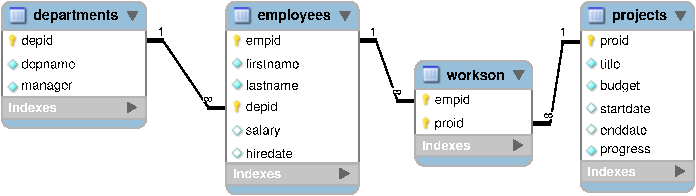
\includegraphics[scale=0.9]{../common/companyREL.pdf}  
\end{minipage}  
\end{frame}



\begin{frame}[t, fragile, shrink]
\frametitle{Πολλά προς πολλά -- βήμα 1}
\begin{minipage}{\wE}
\vspace{-0.5cm}
\begin{block}{\small Σύζευξη {\en\em employees, workson, projects}}
\[
  \begin{split}
      \varrho_{e} (employees) \bowtie_{e.empid=w.empid} \varrho_{w} (workson)  \\
                              \bowtie_{w.proid=p.proid} \varrho_{p} (projects)
  \end{split}
\]
\vspace*{-1em}
\pause
\en
\begin{SQL}
    FROM (employees e INNER JOIN workson w
                         ON e.empid = w.empid)
                      INNER JOIN projects p
                         ON w.proid = p.proid
\end{SQL}
\el  
\end{block}
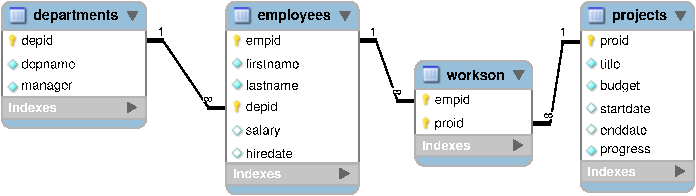
\includegraphics[scale=0.9]{../common/companyREL.pdf}
\end{minipage}
\end{frame}


\begin{frame}[t, fragile, shrink]
\frametitle{Πολλά προς πολλά -- βήμα 2}
\begin{minipage}{\wE}
\vspace{-0.5cm}
\begin{block}{Περιορισμός εγγραφών {\en e.depid=2}}
Υπάρχει o περιορισμός που αφορά τους υπαλλήλους του τμήματος 2:
\[
\begin{split}
    \sigma_{e.depid=2}
    (                           \\
      \varrho_{e} (employees) \bowtie_{e.empid=w.empid} \varrho_{w} (workson)  \\
                              \bowtie_{w.proid=p.proid} \varrho_{p} (projects)
    )
\end{split}
\]
\vspace{-0.5cm}
\pause
\en
\begin{SQL}
    FROM (employees e INNER JOIN workson w
                         ON e.empid = w.empid)
                      INNER JOIN projects p
                         ON w.proid = p.proid
   WHERE e.depid = 2
\end{SQL}
\el
  \end{block}
\end{minipage}
\end{frame}


\begin{frame}[t, fragile, shrink]
\frametitle{Πολλά προς πολλά -- βήμα 3}
\begin{minipage}{\wE}
\vspace{-0.5cm}
\begin{block}{\small Ομαδοποίηση εγγραφών}
Στο ερώτημα υπάρχει ο περιορισμός για ακριβώς 3 συμμετοχές υπαλλήλων σε έργα.
Απαιτείται η εφαρμογή ομαδοποίησης εγγραφών ως προς τα ζητούμενα του ερωτήματος:
\pause
\[
\begin{split}
  {}_{p.proid, p.title} \calg_{count(*)}
    (
      \sigma_{e.depid=2}
      (                           \\
        \varrho_{e} (employees) \bowtie_{e.empid=w.empid} \varrho_{w} (workson)  \\
                                \bowtie_{w.proid=p.proid} \varrho_{p} (projects)
      )
    )
\end{split}
\]
\pause
\vspace{-0.5cm}
\en
\begin{SQL}
    FROM (employees e INNER JOIN workson w
                         ON e.empid = w.empid)
                      INNER JOIN projects p
                         ON w.proid = p.proid
   WHERE e.depid = 2
GROUP BY p.proid, p.title
\end{SQL}
\el
  \end{block}
\end{minipage}
\end{frame}


\begin{frame}[t, fragile, shrink]
\frametitle{Πολλά προς πολλά -- βήμα 4}
\begin{minipage}{\wE}
\vspace{-0.5cm}
\begin{block}{\small Περιορισμός μετά την ομαδοποίηση}
Μετά την ομαδοποίηση των εγγραφών
εφαρμόσουμε τον περιορισμό για ακριβώς 3 συμμετοχές των υπαλλήλων στα έργα:
\[
\begin{split}
  \sigma_{count(*)=3}
  (
    {}_{p.proid, p.title} \calg_{count(*)}
    (
      \sigma_{e.depid=2}
      (                           \\
        \varrho_{e} (employees) \bowtie_{e.empid=w.empid} \varrho_{w} (workson)  \\
                                \bowtie_{w.proid=p.proid} \varrho_{p} (projects)
      )
    )
  )
\end{split}
\]
\pause
\vspace{-0.5cm}
\en
\begin{SQL}
    FROM (employees e INNER JOIN workson w
                         ON e.empid = w.empid)
                      INNER JOIN projects p
                         ON w.proid = p.proid
   WHERE e.depid = 2
GROUP BY p.proid, p.title
  HAVING COUNT(*) = 3
\end{SQL}
\el
  \end{block}
\end{minipage}
\end{frame}


\begin{frame}[t, fragile, shrink]
\frametitle{Πολλά προς πολλά -- Τελική διατύπωση}
\begin{minipage}{\wE}
\vspace{-0.5cm}
\begin{block}{\small Ποια πεδία θέλουμε στο αποτέλεσμα:}
\[
\begin{split}
  \Pi_{p.proid, p.title}
  (
    \sigma_{count(*)=3}
    (
      {}_{p.proid, p.title} \calg_{count(*)}
      (
        \sigma_{e.depid=2}
        (                           \\
          \varrho_{e} (employees) \bowtie_{e.empid=w.empid} \varrho_{w} (workson)  \\
                                  \bowtie_{w.proid=p.proid} \varrho_{p} (projects)
        )
      )
    )
  )
\end{split}
\]
\pause
\vspace{-0.5cm}
\en
\begin{SQL}
  SELECT p.proid, p.title
    FROM (employees e INNER JOIN workson  w
                         ON e.empid = w.empid)
                      INNER JOIN projects p
                         ON p.proid = w.proid
   WHERE e.depid = 2
GROUP BY p.proid, p.title
  HAVING COUNT(*) = 3;
\end{SQL}
\el
\end{block}
\end{minipage}
\end{frame}



